% ---- Writer 3 shared definitions (used by 3.6 - 3.10) ----
\tikzset{
  w3box/.style={draw,rounded corners=2pt,fill=gray!12,align=center,font=\footnotesize,minimum height=8mm,inner sep=3pt},
  w3dark/.style={draw,rounded corners=2pt,fill=gray!30,align=center,font=\footnotesize,minimum height=8mm,inner sep=3pt},
  w3store/.style={draw,fill=white,align=center,font=\footnotesize,minimum height=8mm,inner sep=3pt,double,double distance=1pt},
  w3io/.style={draw,rounded corners=6pt,fill=white,align=center,font=\footnotesize,minimum height=8mm,inner sep=3pt},
  w3dec/.style={draw,diamond,aspect=2.2,fill=white,align=center,font=\scriptsize,inner sep=1pt},
  w3arr/.style={-{Stealth[length=2.2mm]},thick},
  w3dash/.style={-{Stealth[length=2.2mm]},thick,dashed},
  w3group/.style={draw,dashed,rounded corners=4pt,inner sep=5pt},
  w3lab/.style={font=\scriptsize,inner sep=1.5pt}
}

\subsection{Style extraction and glyph library}
\label{sec:styleprofile}

This subsection describes how a writer's style is learned from photographs of that writer's pages and stored permanently (functional units FU~2.5 to FU~2.7; requirements R1 and R6).
``Training'' a writer trains no network.
A \emph{style profile} is built once per writer: a library of the writer's own letter shapes, each reduced to a thin centre-line pen path (a \emph{glyph}), plus measured numbers such as slant, letter height, spacing and how often letters are joined.
It is one text file; afterwards no page images or networks are needed to write in that style.
The builder (Figure~\ref{fig:sty-flow}) is an offline program written by the student, which uses the recogniser of Section~\ref{sec:textrec} for inference only.
Its input is the line crops and transcriptions of Section~\ref{sec:segmentation}: ten pages each of eight database writers (150, 151, 152, 153, 384, 551, 552, 588; the last labelled page is held out, so no evaluation text enters a profile) and the notebook pages of the five personal writers (abhinav, dylan, owen, thiya, yeukita; 15\,\% of their lines held out), aligned with the recogniser fine-tuned on their hands.

\emph{Implementation note: the builder cannot at present extract glyphs from a page image.}
The glyph-extraction function \texttt{ExtractLineGlyphs} of \texttt{Software/\allowbreak CleanPipeline/\allowbreak BuildStyleProfile.py} opens with the statement \texttt{from TrainText import FrameXToPixel,\,INPUT\_WIDTH}, and the recogniser module \texttt{Software/\allowbreak CleanPipeline/\allowbreak TrainText.py} of the delivered pipeline defines no name \texttt{FrameXToPixel} in any spelling: the frame-to-pixel conversion of Equation~\ref{eq:sty-f2p} survives only as the function \texttt{frame\_x\_to\_pixel} of the retired tree \texttt{Software/CNN/TrainText.py}, which was not carried across when the pipeline was rewritten without machine-learning libraries.
Because the statement sits inside the function and not at the top of the module, the module still imports, the profiles already on disk still load, and every cached rebuild and every part of the write path still works; but any fresh extraction of glyphs from a page image raises \texttt{ImportError} at the first line.
The practical consequence is stated plainly: \emph{no new writer can be added and none of the thirteen stored profiles can at present be regenerated from the page images}.
The stored files are dated 10 October 2026 and therefore predate the current state of the code, which is why several of the figures tabulated below had to be re-read from the files themselves rather than reproduced by re-running the builder.
\mustdo{repair the import in \texttt{ExtractLineGlyphs} --- either port \texttt{frame\_x\_to\_pixel} from \texttt{Software/CNN/TrainText.py} into the delivered \texttt{TrainText.py} or compute the conversion of Equation~\ref{eq:sty-f2p} in place --- then re-run the builder on all thirteen writers and confirm that the regenerated profiles match the stored ones.}

\begin{figure}[!htbp]
\centering
\begin{tikzpicture}[x=1cm,y=1cm]
\tikzset{b/.style={w3box,text width=3.05cm,minimum height=1.0cm}}
\node[b] (a1) at (0,0) {Line crop and transcript};
\node[b] (a2) at (3.7,0) {Recogniser: 160 log-probability vectors};
\node[b] (a3) at (7.4,0) {Viterbi forced alignment (Eq.~\ref{eq:sty-viterbi})};
\node[b] (a4) at (11.1,0) {Territories cut at thin low columns (Eq.~\ref{eq:sty-cut})};
\node[b] (b4) at (11.1,-1.6) {Binarise, strip rules, thin whole line};
\node[b] (b3) at (7.4,-1.6) {Trace skeleton, prune spurs, join at junctions};
\node[b] (b2) at (3.7,-1.6) {Split at territories, Douglas--Peucker (Eq.~\ref{eq:sty-dp})};
\node[b] (b1) at (0,-1.6) {Normalise to x-height frame (Eq.~\ref{eq:sty-norm})};
\node[b] (c1) at (0,-3.2) {Quality gates, letter prior (Eq.~\ref{eq:sty-prior})};
\node[b] (c2) at (3.7,-3.2) {Variants, medoid, denoised prototype};
\node[b] (c3) at (7.4,-3.2) {Style statistics (slant, gap, joins)};
\node[w3store,text width=3.05cm,minimum height=1.0cm] (c4) at (11.1,-3.2) {JSON profile, one file per writer};
\foreach \p/\q in {a1/a2,a2/a3,a3/a4,b4/b3,b3/b2,b2/b1,c1/c2,c2/c3,c3/c4,a4/b4,b1/c1} \draw[w3arr] (\p) -- (\q);
\end{tikzpicture}
\caption{Flow chart of the offline style-profile builder: alignment (top), glyph extraction (middle) and profile assembly (bottom).}
\label{fig:sty-flow}
\end{figure}

\subsubsection{Forced alignment: where is each character?}

A character in a joined line has no visible boundary and no per-character labels exist, so \emph{forced alignment} asks which of the recogniser's $T=160$ time steps (4-pixel slices of the canvas) belong to which character, given the known transcript.
Let $y=(y_1,\ldots,y_U)$ be the transcript, $y'=(\varnothing,y_1,\varnothing,\ldots,y_U,\varnothing)$ the blank-augmented label of length $S=2U+1$ (Figure~\ref{fig:rec-ctc}) and $\ell_t(k)=\ln y_t^k$ (Equation~\ref{eq:rec-softmax}).
Where the CTC loss (Equation~\ref{eq:rec-alpha}) \emph{sums} over all paths, the alignment keeps the single best path, found by the Viterbi recursion~\cite{viterbi1967} of Equation~\ref{eq:sty-viterbi}, in which $\delta_t(s)$ is the best log-probability of a path at position $s$ at step $t$:
\begin{equation}
\begin{split}
&\delta_1(1)=\ell_1(\varnothing),\quad\delta_1(2)=\ell_1(y'_2),\quad\delta_1(s)=-\infty\ (s>2),\\
&\delta_t(s)=\ell_t(y'_s)+\max\bigl\{\delta_{t-1}(s),\ \delta_{t-1}(s-1),\ \delta^{\mathrm{skip}}_{t-1}(s)\bigr\},\\
&\delta^{\mathrm{skip}}_{t-1}(s)=\begin{cases}\delta_{t-1}(s-2)&s\ge3,\ y'_s\ne\varnothing,\ y'_s\ne y'_{s-2},\\-\infty&\text{otherwise.}\end{cases}
\end{split}
\label{eq:sty-viterbi}
\end{equation}
The transition that wins the maximum in Equation~\ref{eq:sty-viterbi} is stored as a back-pointer, and the path is traced backwards from its end at a cost of $O(TS)$: it ends on the last character or on the final blank ($s^*_T=S$ if $\delta_T(S)\ge\delta_T(S-1)$, otherwise $s^*_T=S-1$), and character $i$ owns the frames with $s^*_t=2i$, with span $[a_i,b_i)=[t_{\mathrm{first}}-1,t_{\mathrm{last}})$ in frame boundaries.
Figure~\ref{fig:sty-lattice} is a worked example of the lattice and the back-traced path, and is an illustration only; the recursion above is complete.

\begin{figure}[!htbp]
\centering
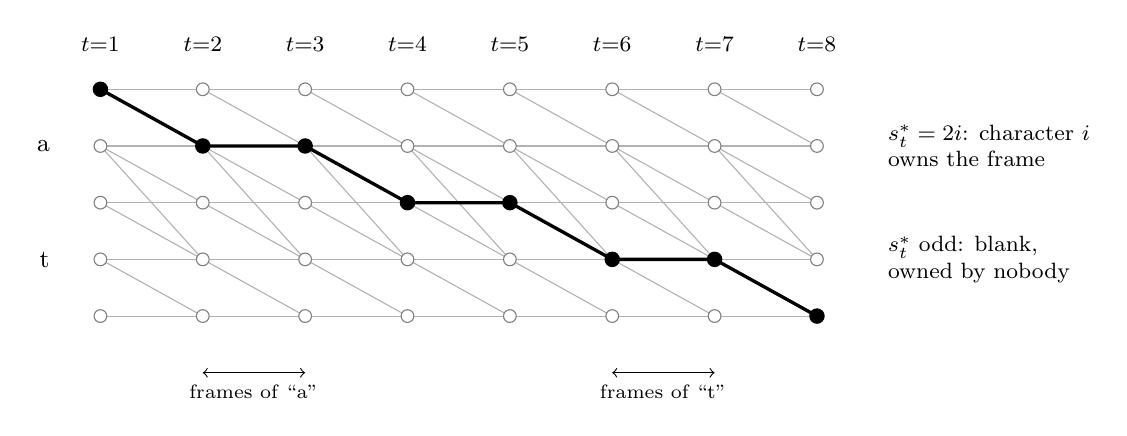
\begin{tikzpicture}[x={(1.3cm,0)},y={(0,-0.72cm)}]
\foreach \t in {1,...,7} {
  \foreach \s in {1,...,5} {\draw[gray!60] (\t,\s) -- (\t+1,\s);}
  \foreach \s in {1,...,4} {\draw[gray!60] (\t,\s) -- (\t+1,\s+1);}
  \draw[gray!60] (\t,2) -- (\t+1,4);
}
\foreach \t in {1,...,8} {\foreach \s in {1,...,5} {\fill[white,draw=gray] (\t,\s) circle (2.3pt);}}
\foreach \s/\l in {1/$\varnothing$,2/a,3/$\varnothing$,4/t,5/$\varnothing$} {\node[font=\small,anchor=east] at (0.6,\s) {\l};}
\foreach \t in {1,...,8} {\node[font=\footnotesize,anchor=south] at (\t,0.5) {$t{=}\t$};}
\draw[very thick] (1,1) -- (2,2) -- (3,2) -- (4,3) -- (5,3) -- (6,4) -- (7,4) -- (8,5);
\foreach \t/\s in {1/1,2/2,3/2,4/3,5/3,6/4,7/4,8/5} {\fill (\t,\s) circle (2.8pt);}
\draw[<->] (2,6.0) -- (3,6.0); \node[font=\scriptsize,anchor=north] at (2.5,6.05) {frames of ``a''};
\draw[<->] (6,6.0) -- (7,6.0); \node[font=\scriptsize,anchor=north] at (6.5,6.05) {frames of ``t''};
\node[font=\footnotesize,anchor=west,align=left] at (8.6,2) {$s^*_t=2i$: character $i$\\ owns the frame};
\node[font=\footnotesize,anchor=west,align=left] at (8.6,4) {$s^*_t$ odd: blank,\\ owned by nobody};
\end{tikzpicture}
\caption{Forced-alignment lattice for the transcript ``at'' with $T=8$ steps (cf.\ Figure~\ref{fig:rec-ctc}). The thick path is the Viterbi path of Equation~\ref{eq:sty-viterbi}; only the frames on the row of a letter belong to that letter, so the spans are narrow.}
\label{fig:sty-lattice}
\end{figure}

\paragraph{Frame-to-pixel conversion and line selection.}
Because the recogniser input is left-aligned with the uniform scale of Equation~\ref{eq:rec-resize}, a frame boundary converts exactly back to a pixel position in the crop: by Equation~\ref{eq:sty-f2p} the frame boundary $a$ lies at the original pixel
\begin{equation}
x_{\mathrm{px}}(a)=\frac{640\,a}{T\,s},\qquad s=\min\Bigl(\frac{64}{h},\frac{640}{w}\Bigr),
\label{eq:sty-f2p}
\end{equation}
for a crop of $h\times w$ pixels, so Equation~\ref{eq:sty-f2p} gives about 6 pixels per frame for a 980-pixel line.
The \emph{alignment confidence} is the mean log-probability along the path, Equation~\ref{eq:sty-conf},
\begin{equation}
\mathrm{conf}=\frac1T\sum_{t=1}^{T}\ell_t\bigl(y'_{s^*_t}\bigr),
\label{eq:sty-conf}
\end{equation}
and the value of Equation~\ref{eq:sty-conf} is low if the recogniser never really read the line, so every line below the 25th percentile of the writer's own confidences is dropped, provided at least eight lines exist: 22 of the 88 lines of writer 153 are discarded in this way.

\paragraph{Cutting the ink into territories.}
CTC spans are narrow slivers that lag the ink, so only their centres $c_k$ (pixels, Equation~\ref{eq:sty-f2p}) are used, with the provisional boundary $\hat x_k=\tfrac12(c_{k-1}+c_k)$ between two characters.
In cursive the only honest boundary is a ligature, where the ink is thin and low, so the boundary is snapped by Equation~\ref{eq:sty-cut} to
\begin{equation}
\begin{aligned}
\mathrm{cost}(x)&=\mathrm{thin}(x)+1.15\,\mathrm{top}(x),\qquad r=\max\bigl(3,\mathrm{round}(0.5x_h)\bigr),\\
x^*&=\arg\min_{|x-\hat x_k|\le r}\Bigl[\mathrm{cost}(x)+0.6\,\frac{|x-\hat x_k|}{r}\Bigr],
\end{aligned}
\label{eq:sty-cut}
\end{equation}
where in Equation~\ref{eq:sty-cut} $\mathrm{thin}(x)$ is the smoothed column ink count divided by its 60th percentile over non-empty columns, $\mathrm{top}(x)$ the height of the highest ink above the baseline in x-heights (limited to 3), the cost is zero in empty columns, and $x_h$ is the x-height of Equation~\ref{eq:wid-xh}.
The cuts are vertical: cutting along the slant lowered the writer identification of the synthesised output from 81.8\,\% to 68.6\,\% (shape classifier, design-stage measurement without raw log), because vertically cut glyphs retile more naturally.

\subsubsection{From ink to ordered pen paths}

\paragraph{Binarisation, core band and slant.}
Each line is binarised like the shape classifier's input (Otsu threshold, rule removal by Equation~\ref{eq:wid-rule}, closing and speck removal; Section~\ref{sec:wid-strokenorm}), and the baseline and x-height $x_h$ come from the core band of Equation~\ref{eq:wid-xh}, whose median over the thirteen writers ranges from 15 to 47 pixels.
The \emph{slant} is the shear that makes the strokes vertical, and it is estimated by the sheared vertical-projection method of Vinciarelli and Luettin~\cite{vinciarelli2001} \mustdo{confirm the page range of the Vinciarelli and Luettin reference (Pattern Recognition Letters, vol.~22, no.~9) in the bibliography; it was left out rather than guessed.}.
For ink pixels $(x_i,y_i)$ with mean row $\bar y$ and trial angle $\theta$ (image $y$ downwards), Equation~\ref{eq:sty-slant} defines the sheared column histogram and its score,
\begin{equation}
x'_i(\theta)=\bigl\lfloor x_i-(y_i-\bar y)\tan\theta\bigr\rfloor,\qquad H_\theta(c)=\#\{i:x'_i(\theta)=c\},\qquad S(\theta)=\sum_cH_\theta(c)^2 ,
\label{eq:sty-slant}
\end{equation}
and $\hat\theta=-\arg\max_\theta S(\theta)$ over $\theta\in\{-45^\circ,-43.5^\circ,\ldots,45^\circ\}$, forward lean positive: since $\sum_cH_\theta(c)$ is fixed, the score of Equation~\ref{eq:sty-slant} peaks when the ink falls in fewest columns.

\paragraph{Thinning and tracing.}
The whole line is thinned \emph{once} with the Zhang--Suen algorithm~\cite{zhang1984} (Equation~\ref{eq:wid-zs}) and only then cut at the territories, because thinning each slice separately creates a spurious spine along the cut.
The skeleton pixels form a graph in the 8-neighbourhood, which is walked into chains: walks start from ends and junctions and follow degree-2 pixels, and chains shorter than 2.5 pixels with a free end are pruned as spurs.
A pen stroke that crosses itself (loops of e, l, o; the bar of t) appears as several chains at a junction, so chain ends within 1.5 pixels of one another are merged repeatedly in order of the smallest continuation angle, the test of Equation~\ref{eq:sty-join},
\begin{equation}
\varphi=\arccos\bigl(-\mathbf d_i\cdot\mathbf d_j\bigr)<75^\circ,
\label{eq:sty-join}
\end{equation}
where $\mathbf d_i,\mathbf d_j$ in Equation~\ref{eq:sty-join} are the outward unit directions of the two ends, so that $\varphi=0$ is a straight continuation.
A chain that crosses a territory boundary is split, and each crossing records that the pen did not lift between the two characters (flags $\mathrm{connL}_i$, $\mathrm{connR}_i$).

\paragraph{Douglas--Peucker simplification.}
Thinning leaves a pixel staircase, so each chain is simplified with the Douglas--Peucker algorithm~\cite{douglas1973}, which recursively splits the chain at the vertex farthest from the chord through its end points $a,b$ until that distance falls below the tolerance $\varepsilon=0.6$ pixels (0.05 to 0.12\,mm at 4\,mm per x-height).
Of a chain with first and last vertex $a,b$, the vertex $p_i$ farthest from the line through $a$ and $b$ has the distance of Equation~\ref{eq:sty-dp},
\begin{equation}
d_i=\frac{\bigl|(b_x-a_x)(p_{i,y}-a_y)-(b_y-a_y)(p_{i,x}-a_x)\bigr|}{\lVert b-a\rVert+10^{-9}},
\label{eq:sty-dp}
\end{equation}
and if $\max_id_i>\varepsilon$ the chain is split there and both halves are simplified recursively, otherwise only $a$ and $b$ are kept; Figure~\ref{fig:sty-dp} sketches the recursion.
\emph{Implementation note:} Equation~\ref{eq:sty-dp} is the distance to the infinite line, not clamped to the segment, so on a closed chain with $a\approx b$ the chord has no length and the whole loop would collapse to two identical points --- which is why the implementation splits closed curves first.
Before the recursion, \texttt{SimplifyPolyline} measures the distance of every vertex from the first, and if the last vertex lies no farther than $\max(1.5,\,0.25\max_i\lVert p_i-p_0\rVert)$ pixels from it the chain is treated as closed, split at its farthest vertex, and the two open halves are simplified separately and rejoined.
The loops of e, l and o are therefore kept.

\begin{figure}[!htbp]
\centering
\begin{tikzpicture}[x=0.82cm,y=0.82cm]
\newcommand{\dppoly}[1]{\draw[#1] (0,0) -- (0.8,0.3) -- (1.5,0.3) -- (2.2,1.2) -- (3.0,1.5) -- (3.8,1.45) -- (4.6,2.0) -- (5.4,1.9) -- (6.0,2.3);}
\dppoly{thick}
\foreach \p in {(0,0),(0.8,0.3),(1.5,0.3),(2.2,1.2),(3.0,1.5),(3.8,1.45),(4.6,2.0),(5.4,1.9),(6.0,2.3)} {\fill \p circle (1.8pt);}
\draw[dashed] (0,0) -- (6.0,2.3);
\draw[gray,dotted] (-0.107,0.280) -- (5.893,2.580);
\draw[gray,dotted] (0.107,-0.280) -- (6.107,2.020);
\draw[<->] (2.2,1.2) -- (2.32,0.889);
\node[font=\scriptsize,anchor=west] at (2.0,0.72) {$d_{\max}>\varepsilon$};
\node[font=\scriptsize,anchor=east] at (-0.15,0) {$a$};
\node[font=\scriptsize,anchor=west] at (6.1,2.3) {$b$};
\node[font=\scriptsize] at (2.2,1.55) {$p_k$};
\node[font=\scriptsize,anchor=north] at (3.0,-0.5) {(a) first split};
\begin{scope}[xshift=8.0cm]
\dppoly{gray}
\draw[very thick] (0,0) -- (1.5,0.3) -- (2.2,1.2) -- (6.0,2.3);
\foreach \p in {(0,0),(1.5,0.3),(2.2,1.2),(6.0,2.3)} {\fill \p circle (2.4pt);}
\node[font=\scriptsize,anchor=north] at (3.0,-0.5) {(b) simplified result};
\end{scope}
\end{tikzpicture}
\caption{Douglas--Peucker simplification (schematic, tolerance exaggerated). (a) The vertex $p_k$ with the largest distance $d_{\max}$ from the chord $ab$ lies outside the tolerance band (dotted) and splits the chain. (b) After recursion on both halves four of the original nine vertices remain.}
\label{fig:sty-dp}
\end{figure}

\paragraph{Normalisation and resampling.}
Every simplified point $(x,y)$ (pixels, $y$ down) of a chain in the territory $[L,R)$ goes, by Equation~\ref{eq:sty-norm}, to the writer-independent frame with baseline 0, $y$ up, unit x-height and the slant removed:
\begin{equation}
y_n=\frac{y_b-y}{x_h},\qquad x_n=\frac{x-L}{x_h}-\sigma\,y_n,\qquad\sigma=\tan\hat\theta .
\label{eq:sty-norm}
\end{equation}
The synthesiser applies the inverse shear (Equation~\ref{eq:syn-place}) to the result of Equation~\ref{eq:sty-norm}, so glyphs are stored upright and re-appear at the writer's lean.
A cursive cut falls inside a ligature, so on a side confirmed connected the outward-running low connector is trimmed, and only if at least 18\,\% of the glyph width remains; the entry and exit points are recorded for the synthesiser's own connector.
Kept variants are then resampled at 0.055 x-heights of arc length and smoothed with two passes of the binomial filter of Equation~\ref{eq:sty-smooth} (end points fixed),
\begin{equation}
q_i\leftarrow\tfrac14q_{i-1}+\tfrac12q_i+\tfrac14q_{i+1}
\label{eq:sty-smooth}
\end{equation}
because without the smoothing of Equation~\ref{eq:sty-smooth} the pixel staircase left by thinning (median turn angle $8.9^\circ$, 90th percentile $59.5^\circ$) would be drawn as hand tremor.

\subsubsection{Variants, quality gates and the cross-writer letter prior}

Of about 2\,122 to 4\,031 raw instances per writer roughly 10\,\% survive five gates, applied per character in order:
(1) \emph{geometry} (size limits, at most six strokes, a class prior on height, no swallowed neighbour, and a pen length above an \emph{adaptive} floor);
(2) \emph{outliers} (width and height within fixed ratios of the 40th-percentile width and the median height);
(3) the \emph{cross-writer prior} of Equation~\ref{eq:sty-prior}, which keeps the 70\,\% nearest;
(4) \emph{consensus}: the nearest 75\,\% to the L1-medoid of the kept descriptors are kept, removing glyphs contaminated by a neighbour;
(5) \emph{typicality}: the best 12 by closeness to the reference width and height are kept.
The pen-length floor of gate~(1) is not a fixed number of x-heights: the live gate is $\max(\texttt{MIN\_PEN\_ABS},\ \texttt{FRAGMENT\_PEN\_FRAC}\cdot\tilde p_c)$ with $\texttt{FRAGMENT\_PEN\_FRAC}=0.5$, $\texttt{MIN\_PEN\_ABS}=0.30$ x-heights and $\tilde p_c$ the median pen length of that character's own instances, because a dotless i is much shorter than an o and a single fixed floor either kept neighbour bleed or discarded real short letters.
(An earlier fixed floor of 1.05 x-heights survives only in the retired tree and is not the gate of the delivered builder.)
\emph{Cross-writer prior.} One writer's ten pages cannot show what a clean letter is; thirteen writers can. A glyph becomes a shape descriptor $v_g$ (points along its strokes accumulated on a $12\times12$ grid over its bounding box, damped, blurred and normalised to unit length); the prior $\bar v_c$ of a character is the normalised element-wise median over all writers, and a glyph's distance is given by Equation~\ref{eq:sty-prior},
\begin{equation}
\mathrm{priorD}(g,c)=1-v_g\cdot\bar v_c\in[0,1].
\label{eq:sty-prior}
\end{equation}
The 70\,\% nearest by Equation~\ref{eq:sty-prior} are kept; the prior only \emph{rejects} malformed variants and later gates substitution, and never imports another writer's shapes.
Two derived glyphs are also stored: the \emph{medoid}, the real variant closest to all others (the writer's own ``ideal'' letter), and a \emph{denoised prototype}, the per-stroke median curve of the modal stroke-count group, which is prepended (so a library can hold 13 variants) only if it is clearly cleaner than the variants it summarises.
Figure~\ref{fig:sty-glyphs} shows stored variants.

\begin{figure}[!htbp]
\centering
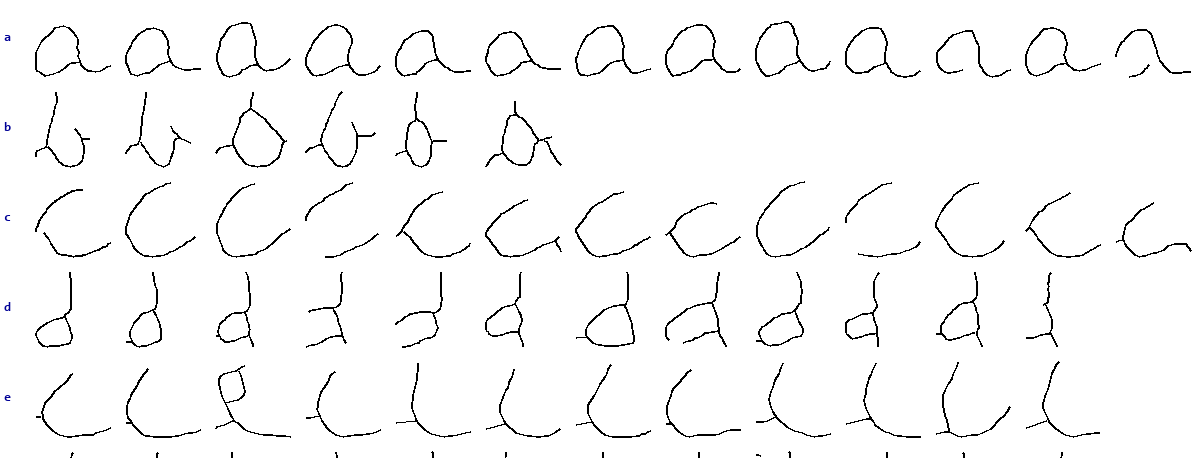
\includegraphics[width=\linewidth]{Figures/w3_glyphs153_ae.png}
\caption{Stored variants of the letters a, b, c, d and e of writer 153 (a strongly joined hand) in the glyph grid of the web interface; each row is one character with up to 12 variants. The short tails at the sides are remains of ligatures.}
\label{fig:sty-glyphs}
\end{figure}

\subsubsection{Style statistics and permanent storage}

Besides glyphs the profile holds numbers measured over the kept lines (Table~\ref{tab:sty-schema} lists every key of a style-profile file with its meaning and an example value from the profile of writer 153): slant, x-height, stroke width, typical ascender and descender reach, the median advance of each character, the word gap, and the \emph{connectedness} of Equation~\ref{eq:sty-conn},
\begin{equation}
c=\frac{\#\{\text{adjacent letter pairs with }\mathrm{connR}\}}{\#\{\text{adjacent letter pairs}\}}.
\label{eq:sty-conn}
\end{equation}
The numerator of Equation~\ref{eq:sty-conn} counts the pen-down crossings recorded during tracing.
The word gap is measured on the \emph{real} ink (median of ink-free column runs wider than $0.5x_h$), because CTC gives a space only a narrow slice, and the slant and reach of the real lines are stored for the calibration of Section~\ref{sec:syn-cal}.

{
\fontsize{9.5}{11.5}\selectfont
\setlength{\tabcolsep}{4pt}
\begin{longtable}{|p{3.2cm}|p{1.6cm}|p{6.6cm}|p{2.5cm}|}
\hline
\textbf{Key} & \textbf{Type} & \textbf{Meaning} & \textbf{Example (153)} \\
\hline
\endfirsthead
\hline
\textbf{Key} & \textbf{Type} & \textbf{Meaning} & \textbf{Example (153)} \\
\hline
\endhead
\hline
\endfoot
\texttt{authorId} & string & Writer identifier. & \texttt{"153"} \\
\hline
\texttt{slantDeg} & float & Median slant of the lines, forward lean positive (Equation~\ref{eq:sty-slant}). & 30.0 \\
\hline
\texttt{xHeightPx} & float & Median pixel x-height of the kept lines. & 33.0 \\
\hline
\texttt{strokeWidthXh} & float & Ink area divided by skeleton length, in x-heights. & 0.189 \\
\hline
\texttt{ascender}, \texttt{descender} & float & Typical reach of tall and descending lower-case glyphs, in x-heights (defaults 1.7 and $-0.6$ if no glyph qualifies). & 1.59, $-1.10$ \\
\hline
\texttt{wordSpaceXh} & float & Word gap measured on the real ink, in x-heights. & 1.59 \\
\hline
\texttt{connectedness} & float & Fraction of adjacent in-word letter pairs that the pen joins (Equation~\ref{eq:sty-conn}). & 0.961 \\
\hline
\texttt{letterAdvance} & dict & Median advance of each character, in x-heights (45 keys). & \texttt{T}: 1.438, \texttt{e}: 1.147 \\
\hline
\texttt{nLines} & int & Number of lines that survived the alignment-confidence cut. & 66 \\
\hline
\texttt{slantMeasRef}, \texttt{ascMeasRef}, \texttt{descMeasRef} & float & Slant (degrees) and ascender and descender reach of the real full lines, measured with the estimators later used on synthesised renders; input of the style calibration (Equation~\ref{eq:syn-cal}). & 30.0, 1.933, $-1.468$ \\
\hline
\texttt{inkFracRef}, \texttt{aspectRef}, \texttt{paperLevel}, \texttt{inkLevel}, \texttt{midFracRef} & float & Ink fraction, width-to-height ratio and grey statistics of the real lines; stored but ignored while the constant pen width is used for rendering. & 0.0620, 14.95, 246, 81, 0.038 \\
\hline
\texttt{glyphs} & dict & Variant library: for each character a list of at most 13 variant dictionaries (37 characters and 283 variants for writer 153). & see below \\
\hline
\texttt{idealGlyphs} & dict & Per-stroke median prototype of a letter (23 characters), with the keys \texttt{strokes}, \texttt{priorD}, \texttt{advance}, \texttt{lead}, \texttt{width}, \texttt{top}, \texttt{bot}, \texttt{entryY}, \texttt{exitY}, \texttt{nPool}. & --- \\
\hline
\texttt{idealMedoid} & dict & The real variant that is most typical of the writer (29 characters), same keys; this is the anchor used by the synthesiser. & --- \\
\hline
\texttt{legibilityLambda} & float & Legibility parameter $\lambda$ of Equations~\ref{eq:syn-global} and~\ref{eq:syn-swap}; written by the tuner after the build, \emph{not} by the builder. \textbf{Absent from all thirteen stored profiles}, so the deployed code falls back to $\lambda=0$ (see below). & not present \\
\hline
\multicolumn{4}{|l|}{\textbf{Keys of one variant in \texttt{glyphs[c][i]}}} \\
\hline
\texttt{char} & string & The character. & \texttt{"e"} \\
\hline
\texttt{strokes} & list & Strokes, each a list of $[x,y]$ points in x-height units, baseline $y=0$, upright. & 2 strokes, 4 and 33 points \\
\hline
\texttt{width}, \texttt{advance}, \texttt{lead} & float & Ink width, cell width and gap before the ink, in x-heights. & 0.903, 1.097, 0.0 \\
\hline
\texttt{top}, \texttt{bot} & float & Highest and lowest point. & 0.871, 0.0 \\
\hline
\texttt{entryX}, \texttt{entryY}, \texttt{exitX}, \texttt{exitY} & float & Entry and exit points of the pen for connectors. & $-0.149$, 0.258, 0.847, 0.097 \\
\hline
\texttt{connL}, \texttt{connR} & bool & The pen was joined to the left or right neighbour. & true, true \\
\hline
\texttt{priorD} & float & Cosine distance to the cross-writer letter prior (Equation~\ref{eq:sty-prior}). & 0.1179 \\
\hline
\texttt{denoised} & bool & Present and true if the variant is the denoised prototype. & --- \\
\hline
\caption{Keys of a style-profile file (JavaScript Object Notation). The example column was re-read from the stored file \texttt{StyleProfiles10/153.json}; an earlier version of this table quoted the values of a superseded build of that profile.}
\label{tab:sty-schema}
\end{longtable}
}

The thirteen writers differ widely (Table~\ref{tab:sty-writers}, which lists the scalar values of all thirteen stored profiles, re-read from the files themselves): slant from $-10.5^\circ$ to $42.0^\circ$, connectedness 0.195 to 0.968, word gap 0.94 to 2.68 x-heights, the diversity requirement R1 asks the system to reproduce.

\begin{table}[!htbp]
\centering
\fontsize{9}{11}\selectfont
\setlength{\tabcolsep}{3pt}
\begin{tabular}{|l|r|r|r|r|r|r|r|r|r|r|r|}
\hline
\textbf{Writer} & \textbf{Lines} & \textbf{Slant ($^\circ$)} & \textbf{$x_h$ (px)} & \textbf{Stroke width} & \textbf{$A$} & \textbf{$D$} & \textbf{Gap} & \textbf{Conn.} & \textbf{$\lambda$} & \textbf{Chars} & \textbf{Var.} \\
\hline
150 & 61 & $-4.5$ & 47 & 0.096 & 1.58 & $-0.72$ & 1.33 & 0.343 & 0.90$^\dagger$ & 42 & 296 \\
151 & 58 & 33.0 & 22 & 0.271 & 2.69 & $-1.09$ & 1.59 & 0.968 & 1.00$^\dagger$ & 43 & 287 \\
152 & 59 & 19.5 & 46 & 0.104 & 1.48 & $-0.79$ & 1.47 & 0.715 & 0.45$^\dagger$ & 38 & 273 \\
153 & 66 & 30.0 & 33 & 0.189 & 1.59 & $-1.10$ & 1.59 & 0.961 & 0.45$^\dagger$ & 37 & 283 \\
384 & 54 & 4.5 & 43 & 0.107 & 1.93 & $-0.71$ & 1.37 & 0.500 & 0.30$^\dagger$ & 36 & 252 \\
551 & 58 & 42.0 & 20 & 0.225 & 1.84 & $-0.67$ & 2.68 & 0.557 & 1.00$^\dagger$ & 38 & 271 \\
552 & 47 & $-10.5$ & 32 & 0.148 & 1.62 & $-0.56$ & 1.53 & 0.609 & 0.00$^\dagger$ & 40 & 288 \\
588 & 58 & 0.0 & 29 & 0.163 & 1.73 & $-0.68$ & 2.07 & 0.668 & 0.30$^\dagger$ & 41 & 254 \\
abhinav & 130 & 6.0 & 28 & 0.141 & 1.78 & $-0.84$ & 2.13 & 0.789 & --- & 56 & 335 \\
dylan & 79 & $-6.0$ & 26 & 0.135 & 1.68 & $-0.62$ & 1.79 & 0.195 & 1.00$^\dagger$ & 42 & 302 \\
owen & 93 & 0.0 & 32 & 0.111 & 1.51 & $-0.68$ & 1.10 & 0.319 & --- & 43 & 307 \\
thiya & 48 & 30.75 & 15 & 0.331 & 2.24 & $-1.00$ & 1.65 & 0.962 & --- & 42 & 239 \\
yeukita & 74 & 0.0 & 27 & 0.151 & 1.45 & $-0.58$ & 0.94 & 0.417 & 0.15$^\dagger$ & 58 & 333 \\
\hline
\end{tabular}
\caption{Scalar values of the thirteen stored style profiles, read directly from the files in \texttt{Software/CNN/NOGIT/StyleProfiles10}: kept lines, slant, pixel x-height, stroke width (x-heights), ascender $A$ and descender $D$ and word gap (x-heights), connectedness, legibility parameter $\lambda$, number of characters and number of variants. Writers 150 to 588 are database writers, the last five are the personal writers. $^\dagger$The $\lambda$ column is \emph{not} read from these files: the key \texttt{legibilityLambda} is absent from every one of them, and the values shown are the output of an earlier tuning run that predates the current profiles; abhinav, owen and thiya were added afterwards and were never tuned. An earlier version of this table listed ten writers and the scalar values of a superseded build.}
\label{tab:sty-writers}
\end{table}

\paragraph{The legibility parameter is not in the stored profiles.}
The legibility parameter $\lambda$ (Section~\ref{sec:synthesis}) is written into the file after the build by the tuner \texttt{TuneLegibility} of \texttt{Evaluate.py}, not by the builder, and \emph{the key is absent from all thirteen files as delivered}: the profiles were rebuilt after the tuner last ran and the tuner was not re-run on them.
Every reader of the key in the synthesiser supplies a default when it is missing, and the default on the deployed path is zero --- the server calls \texttt{SynthesizeJointBestOf}, which takes \texttt{profile.get('legibilityLambda',\,0.0)} --- so \emph{the delivered system synthesises every writer at $\lambda=0$}, that is, entirely from the writer's own glyphs with no legibility anchor substitution at all.
(One older entry point, \texttt{SynthesizeLegible}, falls back to \texttt{DEFAULT\_LEGIBILITY}${}=0.65$ instead, but the server does not use it.)
The $\lambda$ values of Table~\ref{tab:sty-writers} are genuine measurements of the tuning run that produced them and are retained for that reason, but they describe neither the stored profiles nor the behaviour of the delivered system, and the design-stage gains attributed to per-writer $\lambda$ in Section~\ref{sec:synthesis} are therefore not realised by the code as submitted.
\mustdo{re-run \texttt{TuneLegibility} over the thirteen current profiles so that \texttt{legibilityLambda} is written back into each file, then re-measure the figures of Table~\ref{tab:syn-evid} that depend on it; until this is done the per-writer legibility control described in Section~\ref{sec:synthesis} is inactive.}

\emph{Permanent storage (R6):} a profile is a JavaScript Object Notation (JSON) text file of 290 to 497\,kB (about 4.8\,MB for all thirteen), loaded when the server starts (Section~\ref{sec:system}); thirteen profiles exist and the web interface lists them.
\mustdo{the demonstration of R6 (display of the stored writers, reproduction in a writer chosen by the examiner) and the storage device holding the files.}

\subsubsection{Design alternatives and justification}

Table~\ref{tab:sty-alt} lists the alternatives with the reason for the chosen design.
Fixed widths, projection minima or hand labelling would replace the forced alignment, but joined letters have no gaps, hand labelling of about 90 pages is impractical, and the recogniser already knows the text.
One averaged letter per writer blurs letters whose strokes are arranged differently, whereas variants keep the natural variation; importing the median shape into every writer would erase the writer, whereas filtering keeps the shapes the writer's own; and a generator learned from on-line pen data is impossible, because no such data exist for the thirteen writers (47 to 130 usable lines each).
Cutting a joined line destroys how a letter changes with its neighbours, so the most joined hands (writers 151 and 551) are reproduced least legibly (Section~\ref{sec:synthesis}).

\begin{table}[!htbp]
\centering
\fontsize{9.5}{11.5}\selectfont
\begin{tabularx}{\linewidth}{|p{3.0cm}|X|X|}
\hline
\textbf{Decision} & \textbf{Alternative} & \textbf{Reason for the chosen design} \\
\hline
Character boundaries & Fixed widths, projection minima, hand labelling. & Joined letters have no gaps and hand labelling of about 90 pages is impractical; the recogniser knows the text, so alignment is automatic. \\
\hline
Thin whole line, then cut & Thin each slice. & A slice edge creates a spurious spine stored as a bar. \\
\hline
Several variants per letter & One averaged letter. & Averaging blurs letters whose strokes are arranged differently; variants keep the natural variation, medoid and prototype remain options. \\
\hline
Prior as a filter & Import the median shape into every writer. & Importing would erase the writer; filtering keeps the shapes the writer's own. \\
\hline
Glyphs from scanned pages & Generator learned from on-line pen data. & No on-line data of the thirteen writers exist (47 to 130 usable lines each), and the pen path must be recovered from the image in any case (Section~\ref{sec:synthesis}). \\
\hline
\end{tabularx}
\caption{Design alternatives for the style extraction.}
\label{tab:sty-alt}
\end{table}

A real example of the builder stages, Figure~\ref{fig:sty-stages}, is still to be supplied.

\begin{figure}[!htbp]
\centering
\figplaceholder{3.4cm}{One real line of a database writer and one personal line: grey crop, ink mask with rules removed and core band, Zhang--Suen skeleton, traced chains in colours with the territory cuts as vertical lines, and one extracted glyph in the normalised frame. Source: the functions of the profile builder applied to a crop of \texttt{Data/Datasets/IAMpages10} and one of \texttt{Software/CNN/NOGIT/dylan}.}
\caption{Stages of the style builder on real lines (placeholder).}
\label{fig:sty-stages}
\end{figure}
